% Migrated from the Word baseline; do not duplicate content in other section files.
\section{数值实验与结果}\label{sec:numerical-results}

\subsection{实验目的、数值模型与评价方法}\label{sec:numerical-6-1}

数值实验依次检验低维网络实现、固定 \(N_{\mathrm{diag}}=2\) 诊断基上的学习行为，以及 COMSOL--Galerkin canonical 数据映射的一致性。P0 采用四维非线性耦合振子，对比普通向量场网络、Real HNN、标准复线性 CHNN 和广义复线性 CHNN。P1、P1.5 和 P1.6 采用 mode1、mode2、mixed12 三条固定轨迹，分别考察导数监督、灰箱 residual 和平衡硬约束；每次测试均留出一条完整轨迹，五个随机种子仅表示算法重复，不作为独立物理样本。canonical 数据映射实验则用于诊断坐标、余切动量和广义力标签中的误差来源；现有单一哨兵至多是后续 A1 资格实验的候选输入，不认证多幅值或跨工况数据生成资格。

评价量包括向量场相对 L2 误差、rollout 误差、线性化误差、能量漂移、canonical 闭合误差和时间离散收敛阶。Bridge 扰动能量门与 force-v2 联合 L2 门分别回答能量漂移和力闭合问题，采用彼此独立的阈值。当前交付物缺少可复核的原始数组、指标函数、切片和阈值来源，因此这些名称和历史摘录不能被重新计算为完整 G0--G6 机器门。训练、验证和测试数据按完整参数工况划分，而不是从同一轨迹中随机抽点；但 fold manifest、早停和归一化日志尚未交付。完整的 96 轨迹数据集、P2 模型比较、开放端口、高保真偏差和数值 KAM 检验属于后续数值研究，本节不把当前小样本结果外推到这些问题。

\subsection{数值实现与 COMSOL--Galerkin bridge}\label{sec:numerical-6-2}

数值实现通过了源文件编译、可编辑安装、组件与接口测试以及合成数据训练流程检验。独立进程中的 13 个回归测试文件连续运行三轮均未出现失败。这些测试用于检查软件实现的一致性，不作为模型科学性能的证据。

COMSOL--Galerkin bridge 包含 stationary 导出、mesh-40/80 模态现实性检查、前 12 个候选模态以及三条 \(1\,\mathrm{s}\) 候选轨迹。原扰动能量判据采用 \(0.5\%\) 阈值，仅 mode2 满足；若采用探索性的 \(1\%\) 阈值，则三条轨迹均满足。force-v2 在公共支持 indices \(2\ldots998\) 和固定 \(p[2]\) 锚点下，以独立的 \(2\%\) 联合 L2 阈值检验力闭合，三条轨迹均满足。\Cref{tab:bridge-gate-summary,fig:bridge-gate-separation}分别报告这些判据，避免把能量门与力门合并解释。

\begin{table}[htbp]
\centering
\caption{Bridge 扰动能量与 force-v2 力闭合的逐轨迹比较。能量漂移分别采用 \(0.5\%\) 判据和探索性的 \(1\%\) 判据；force-v2 使用独立的联合 L2 判据。}
\label{tab:bridge-gate-summary}
\scriptsize
\setlength{\tabcolsep}{4pt}
\begin{tabular}{@{}lccccc@{}}
\toprule
轨迹 & 扰动能量漂移（\%） & \(<0.5\%\) & \(<1\%\) & force-v2（\%） & \(<2\%\) \\
\midrule
mode1  & 0.815090 & 失败 & 通过 & 1.513677 & 通过 \\
mode2  & 0.329369 & 通过 & 通过 & 0.062551 & 通过 \\
mixed12 & 0.523328 & 失败 & 通过 & 1.080748 & 通过 \\
\bottomrule
\end{tabular}
\end{table}


\begin{figure}[htbp]
\centering
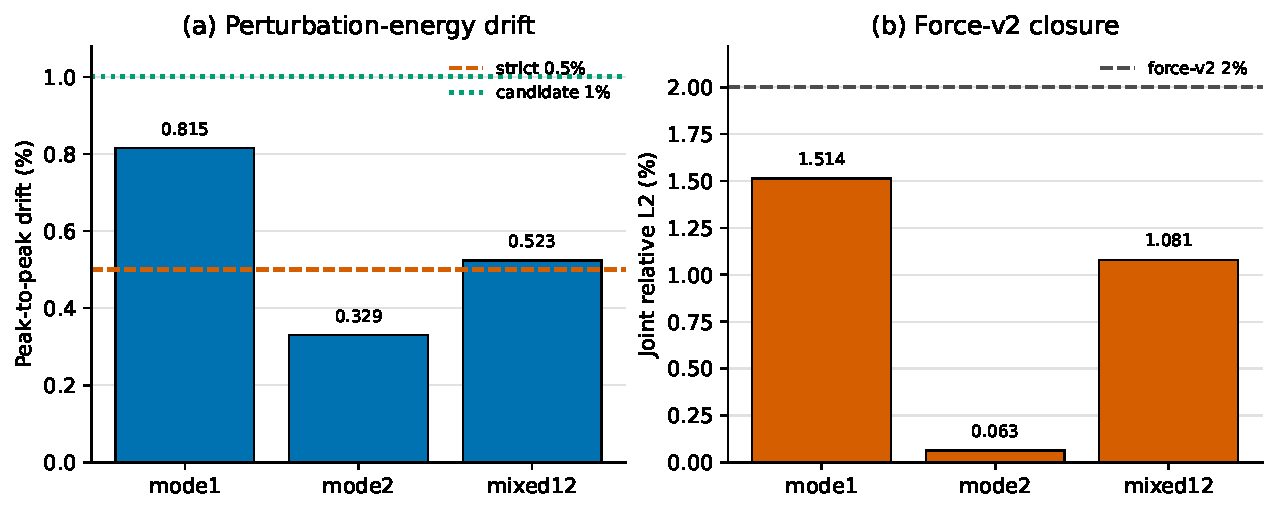
\includegraphics[width=0.94\linewidth]{figures/fig_bridge_gate_separation.pdf}
\caption{Bridge 扰动能量判据与 force-v2 力闭合判据。左图对同一扰动能量漂移分别标出 \(0.5\%\) 判据和探索性的 \(1\%\) 判据；右图给出 force-v2 联合 L2 误差及其独立的 \(2\%\) 阈值。}
\label{fig:bridge-gate-separation}
\end{figure}

\subsection{保守分支辨识结果}\label{sec:numerical-6-3}

\subsubsection{P0 低维架构基线}\label{sec:numerical-6-3-p0}

P0 在统一的四维耦合振子上采用 \(80/16/20\) 条训练/验证/测试轨迹，每条轨迹 80 步，\(\Delta t=0.025\)，训练 300 epochs，并使用五个算法种子。包含 quadratic physics baseline 时，标准 CHNN 的向量场和 rollout 相对 L2 分别为 \(0.0109144\) 和 \(0.0351959\)，低于 Real HNN 的 \(0.0122422\) 和 \(0.0444270\)；其能量漂移 \(0.00455759\) 则不低于 Real HNN 的 \(0.00402084\)。因此，该实验支持低维实现和架构比较，但不能替代 COMSOL 数据上的 P2 比较或 KAM 检验。

\begin{table}[htbp]
\centering
\caption{P0 quadratic-physics 分支的模型比较。向量场网络不使用 physics baseline。}
\label{tab:p0-summary}
\small
\begin{tabular}{@{}lccc@{}}
\toprule
模型 & 向量场相对 L2 & rollout 相对 L2 & 能量漂移 \\
\midrule
向量场网络 & 0.0200837 & 0.103076 & 0.0245256 \\
Real HNN & 0.0122422 & 0.0444270 & 0.00402084 \\
标准 CHNN & \textbf{0.0109144} & \textbf{0.0351959} & 0.00455759 \\
广义复线性 CHNN & 0.0121700 & 0.0458872 & 0.00403167 \\
\bottomrule
\end{tabular}
\end{table}


\subsubsection{P1、P1.5 与 P1.6}\label{sec:numerical-6-3-p1}

P1 的 \(60/60\) 次运行均完成。在三条 held-out 轨迹上，标准 CHNN 的联合向量场相对误差为 \(0.1417\%\)--\(0.2444\%\)，rollout 误差为 \(0.2131\%\)--\(1.5237\%\)，线性化误差为 \(0.3125\%\)--\(0.3286\%\)；在该小样本实验的五个算法种子比较中，其联合场、rollout 和线性化指标相对三个基线均有 \(15/15\) 次较低。该结论只适用于三条固定小轨迹和 derivative-only 目标。

P1.5 的 \(60/60\) 次运行也均完成。相对 physics-only，residual 模型的联合场平均降幅为 \(90.37\%\)--\(97.29\%\)，rollout 平均降幅为 \(53.40\%\)--\(95.14\%\)。标准 CHNN 相对灰箱 Real HNN 的联合场在 \(11/15\) 次运行中较低，但平均相对降幅为 \(-2.195\%\)；rollout 在 \(12/15\) 次运行中较低且平均降幅为 \(20.915\%\)，代价约为 \(3.04\times\) 训练时间和 \(2.54\times\) 评估时间。这表明其收益具有指标依赖性，并不构成稳定的一步向量场优势。

P1.6 的 \(30/30\) 个硬约束模型均以零数值残差满足 \(f(0)\) 和零点 Jacobian 条件，但预测精度显著恶化：Real HNN 的联合场/rollout 均值从 \(1.832\times10^{-3}/1.439\times10^{-2}\) 变为 \(2.872\times10^{-2}/1.011\times10^{-1}\)，标准 CHNN 从 \(1.819\times10^{-3}/1.195\times10^{-2}\) 变为 \(2.623\times10^{-2}/7.594\times10^{-2}\)。因此，精确满足平衡约束并不必然改善预测性能。\Cref{tab:p1-series-summary}汇总了三组实验的主要结果和适用边界。

\begin{table}[htbp]
\centering
\caption{P1 系列结果与解释边界。五个 seed 均为算法重复，物理轨迹数始终为三。}
\label{tab:p1-series-summary}
\small
\begin{tabularx}{\textwidth}{@{}l>{\raggedright\arraybackslash}X>{\raggedright\arraybackslash}X@{}}
\toprule
实验 & 数值结果 & 适用范围 \\
\midrule
P1 &
标准 CHNN 的联合场、rollout、线性化误差分别为 \(0.1417\%\)--\(0.2444\%\)、\(0.2131\%\)--\(1.5237\%\)、\(0.3125\%\)--\(0.3286\%\)。 &
仅适用于三条轨迹的 derivative-only 小样本比较。 \\
P1.5 &
residual 相对 physics-only 的场/rollout 平均降幅为 \(90.37\%\)--\(97.29\%\)/\(53.40\%\)--\(95.14\%\)；CHNN 对 gray Real 的场平均降幅为 \(-2.195\%\)。 &
收益有条件且计算更贵；不支持稳定一步场优势。 \\
P1.6 &
\(30/30\) 个约束模型精确通过平衡门，但 Real/CHNN 联合场均值分别恶化至 \(2.872\times10^{-2}\)/\(2.623\times10^{-2}\)。 &
约束满足不等于精度改善。 \\
\bottomrule
\end{tabularx}
\end{table}


\subsubsection{Canonical 数据合同诊断与时间步收敛}\label{sec:numerical-6-3-contract}

初始检查中，跨轨迹比较造成了一次假阳性；采用同轨迹比较后，mode1 满足判据，而 mixed 仍未满足。重复的单一 mode1 工况同样可能出现闭合误差，说明模态混合不是异常的必要条件。进一步比较排除了 \(N_{\mathrm{diag}}=2\) 诊断截断不足这一解释，并显示投影动量的闭合优于 \(M_N\dot q_{\mathrm{native}}\)。generalized-alpha 的内部 stage 无法通过公共 API 直接取得，因此不能保证坐标、动量和力标签属于同一内部求解阶段；改用二阶 BDF 的 \texttt{tsteps} 输出后，可以保存同一 solver step 上的 canonical 状态。这里的 BDF 仅用于状态采样和向量场标签生成，并未被证明为辛积分器。

随后发现，mixed 初值没有应用固定基的 normalization/sign transform。对位移与速度统一实施该变换后，离线初值一致性检查 \(12/12\) 满足，mixed 短时间窗的 canonical 闭合也满足预设条件。初始的双层时间步比较中，G2 从 \(0.00147337\) 增至 \(0.00155680\)，未满足预设的单调收敛判据，因此进一步引入第三层时间步进行澄清。

历史三层表格中的动量率行现标为含输运项的 \(\dot p_N\) proxy；由于尚未交付 \(B_N,\dot B_N,P_{\mathrm{full}}\) 原始数组和实现，该行不能作为 canonical 合同的新验证。冻结记录报告的观察阶范围为 \(1.64186\)--\(2.00088\)，随后 \(1\,\mathrm{s}\) mode1\_phi\_pio2 工况报告 G2、G3 点态、G3 impulse 和扰动能量峰峰漂移分别为 \(0.00146226\)、\(0.000221162\)、\(0.0000563606\) 和 \(0.00307057<0.005\)。这些历史数值仍待输运修正映射实现后重算；\Cref{tab:canonical-time-step,fig:b0-r2-convergence-orders}给出冻结记录。

\begin{table}[htbp]
\centering
\caption{Canonical 数据合同的三层收敛与 \(1\,\mathrm{s}\) 验证结果。}
\label{tab:canonical-time-step}
\small
\begin{tabular}{@{}llcc@{}}
\toprule
工况 & 指标 & 数值 & 判据/结论 \\
\midrule
三层 & \(q\) 观察阶 & 1.9978492 & 通过 \\
三层 & \(p_{\mathrm{projected}}\) 观察阶 & 2.0008768 & 通过 \\
三层 & \(M_N^{-1}p\) 观察阶 & 2.0008769 & 通过 \\
三层 & \(B^{T}L\) 观察阶 & 1.9976914 & 通过 \\
三层 & total energy 观察阶 & 1.6418624 & 通过 \\
\midrule
\(1\,\mathrm{s}\) & G2 联合相对 L2 & 0.00146226 & \(<0.02\) \\
\(1\,\mathrm{s}\) & G3 点态相对 L2 & 0.000221162 & \(<0.02\) \\
\(1\,\mathrm{s}\) & G3 impulse 相对 L2 & 0.0000563606 & \(<0.02\) \\
\(1\,\mathrm{s}\) & 扰动能量峰峰漂移 & 0.00307057 & \(<0.005\) \\
\bottomrule
\end{tabular}
\end{table}


\begin{figure}[htbp]
\centering
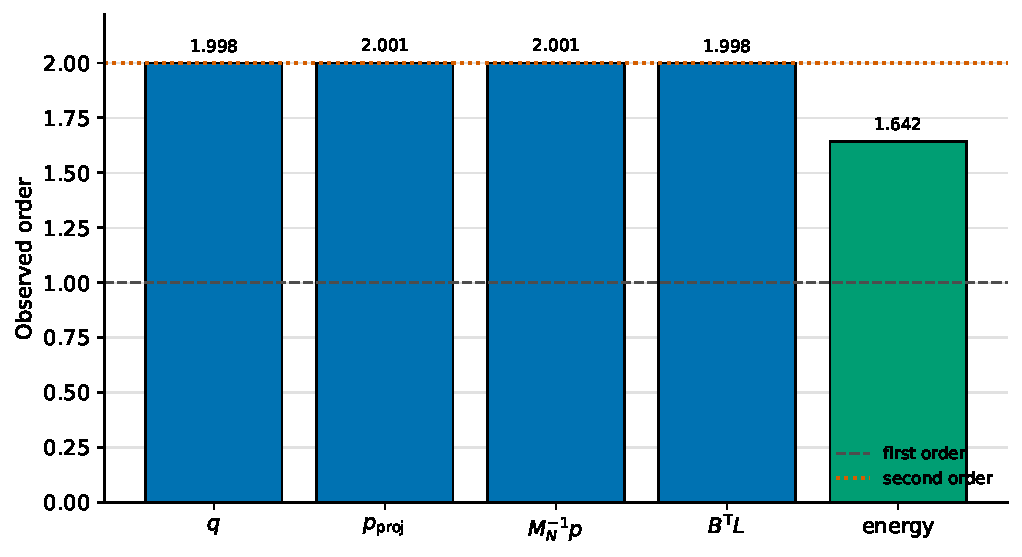
\includegraphics[width=0.88\linewidth]{figures/fig_b0_r2_convergence_orders.pdf}
\caption{Canonical 数据合同三层时间离散比较的观察收敛阶。所考察量的收敛阶为 \(1.64186\)--\(2.00088\)，均高于一阶；该结果不用于证明 BDF 的辛性或给出 KAM 数值认证。}
\label{fig:b0-r2-convergence-orders}
\end{figure}

当前有限证据至多支持该单一诊断哨兵作为后续 A1 资格实验的候选输入；它不认证跨 mode、幅值或工况的数据生成资格。多幅值统计、完整 96 轨迹构建及正式 P2 模型比较将在后续实验中给出；当前结果尚不能证明 CHNN 在该完整任务上普遍优于 Real HNN。

\subsection{开放端口与高保真数值验证方案}\label{sec:numerical-6-4}

开放端口分支将在配对工况和消融实验下比较状态预测误差、分项广义力误差、功率平衡残差、耗散符号违反率、端口泄漏指标和长期轨迹误差，以检验保守力、耗散力和外部端口的可辨识性。高保真对照将量化 Kirchhoff 主模型相对 Timoshenko 梁和实体模型的偏差。相关实例化计算尚待完成，因此本节仅规定比较方法和评价量，不给出模型优劣结论。

\subsection{高阶误差证书与数值 KAM 验证方案}\label{sec:numerical-6-5}

数值 KAM 研究需要进一步确定主模态阶数、可积参考系统和正规形系数，并计算频率映射非退化裕度、有限阶 Diophantine 裕度、高阶或解析误差证书、辛映射缺陷、步长非共振条件及不变环面残差。只有当总误差与所选 KAM 定理阈值在同一范数下可比较时，才能讨论数值认证。当前 canonical 闭合与时间步收敛结果并不构成 KAM 数值认证，也尚未获得不变环面。

\subsection{参数延拓、模型偏差与安全操控域}\label{sec:numerical-6-6}

后续研究将沿磁场强度、推进速度、流速、接触间隙和材料参数进行延拓，同时报告结构响应、端口指标以及低阶与高保真模型之间的偏差。完整工程安全域还需综合开放端口功率交换、接触峰值、高保真模型偏差和不确定性传播，不能与保守 KAM 骨架的理论保证域等同。由于这些计算尚未实例化，本文不宣称已经获得工程安全域。
